%%!TEX encoding = UTF-8 Unicode

% Several lines in file have comments suggesting common packages for the
% typical thesis in informatics or electronics developed at UA
% uncomment/comment the lines as required for your work
% Before each optional line you will have a small comment

% According to UA rules, font size should range from 10 to 12pt.
\documentclass[11pt,a4paper,openright,twoside,onecolumn]{memoir}

\listfiles
\fixpdflayout

\usepackage[utf8]{inputenc}

% Select Computer Modern Typewritter (For bold ttfamily in listings)
\usepackage{lmodern}
% OR... Bera Mono
%\usepackage[scaled]{beramono} % TTT Font
%\usepackage{anyfontsize} % As the name says...

\usepackage[T1]{fontenc}

% Enable for for Overleaf support
\usepackage{ifthen}
\def\useoverleaf{0}  % change to non-zero (for instance, 1) to enable it

\makeatletter
\newcommand{\makecoverfile}[0]{%
  \immediate\write18{latexmk -pdf cover.tex}%
}
\makeatother

% For PDF merging
\usepackage{pdfpages}

% Set DPI to 300
\pdfpxdimen=\dimexpr 1in/300\relax

% Allow the use of a larger number of packages
\usepackage{morewrites} 

% For English and Portuguese languages
% Portuguese will be the default.
% Uncomment \setlanguage below to change it
\usepackage[english,portuguese]{babel}

% Uncomment to use a custom date format
%\usepackage{datetime}
%\newdateformat{thesisdate}{\monthname[\THEMONTH] \THEYEAR} % Month Year

% Make pdf look better
\usepackage{microtype} 

% Uncomment to enable floats on facing pages
%\usepackage{dpfloat}

% Side by side figures
% Eg. Fig 1a, Fig 1b
\usepackage[hang,small,bf]{caption}
%\let\tion\undefined
%\let\subfloat\undefined
\usepackage{subcaption}

%\RequirePackage{textcase}

% Dropped Caps
%\usepackage{lettrine}

% Configure Hyperlink color
% As a matter or style, you may use this to enable/disable color boxes on links
%\usepackage[breaklinks=true,colorlinks=false,linkcolor=blue]{hyperref}
% Or use the default values provided by the hyperref package
\usepackage{hyperref}

% Redefine section names according to your preference
%\def\sectionautorefname{Section}
%\def\chapterautorefname{Chapter}
%\def\figureautorefname{Figure}
%\def\listingautorefname{Listing}
%\def\tableautorefname{Table}

% Redefine code boxes
\ifthenelse{\equal{\useoverleaf}{0}}
{\usepackage[outputdir=build]{minted}}
{\usepackage{minted}}%

\addto\captionsportuguese{%
  \renewcommand\listingscaption{Código}
}
\fvset{fontsize=\footnotesize} % Make Code blocks smaller than text
\usepackage{csquotes}

% Add support for PDF Comments
\usepackage{comment}
\ifthenelse{\equal{\useoverleaf}{0}}
{\usepackage{pdfcomment}}{}
\usepackage{bookmark} % New Bookmarks

% For Multiple columns in Glossary
\usepackage{multicol}

% Add support for Math symbols
\usepackage{amsmath}
\usepackage{amssymb}

% Add support for graphics
\usepackage{graphicx}

% Add support for Colors
\usepackage{xcolor}

% Add support for the Euro symbol
\usepackage{eurosym}

% Add support for missingfigure and todo
\usepackage{todonotes}

% Setup bibliography with Biber using IEEE style for proper UTF-8 support
\usepackage[backend=biber, style=ieee, sorting=none, natbib=true, mincitenames=1, maxcitenames=2]{biblatex}
\bibliography{bib/references.bib, bib/rfc.bib}

% Use acronyms
\usepackage[printonlyused]{acronym} % For acronyms

% Indenting the first paragraph after section start
\usepackage{indentfirst}

% For fixing listoflistings with memoir
\usepackage{xparse}

% To enumerate with letters
\usepackage{enumitem}

% Uncomment the next lines to enable chart support through pgf and tikz
% This may require you to install further packages in your Tex system
%\usepackage[version=0.96]{pgf}
%\usepackage{tikz}

% UML support
%\usepackage{pgf-umlsd}

% Trees, Arrows, Mindmaps and other popular objects
%\usetikzlibrary{arrows,shadows,trees,shapes,decorations,automata,backgrounds,petri,mindmap} % for pgf-umlsd

% Package to master SI units
\usepackage[detect-weight=true, binary-units=true]{siunitx}
% For Electric Circuits
%\sisetup{load-configurations = binary}

% Set Voltage direction accordingly
% Option : oldvoltagedirection,nooldvoltagedirection,RPvoltages,EFvoltages
% More information at: https://mirrors.ibiblio.org/CTAN/graphics/pgf/contrib/circuitikz/doc/circuitikzmanual.pdf
% By default this template is using the Old Voltage Direction
%\usepackage[oldvoltagedirection,american,cuteinductors,smartlabels]{circuitikz}
%\usetikzlibrary{calc}
%\ctikzset{bipoles/thickness=1}
%\ctikzset{bipoles/length=0.8cm}
%\ctikzset{bipoles/diode/height=.375}
%\ctikzset{bipoles/diode/width=.3}
%\ctikzset{tripoles/thyristor/height=.8}
%\ctikzset{tripoles/thyristor/width=1}
%\ctikzset{bipoles/vsourceam/height/.initial=.7}
%\ctikzset{bipoles/vsourceam/width/.initial=.7}
%\tikzstyle{every node}=[font=\small]
%\tikzstyle{every path}=[line width=0.8pt,line cap=round,line join=round]

% For inline TT text (e.g. code snippets)
\usepackage{verbatim}

% Frames around figures and allow force placement
\usepackage{float}

% Configure Float style
%\floatstyle{boxed}
%\restylefloat{table}
%\restylefloat{figure}
%\restylefloat{lstlisting}

% For test purposes you may use the lipsum package to create dummy text
\usepackage{lipsum} % REMOVE

%Keep floats inside section!
\usepackage[section]{placeins}
\let \oldsubsubsection \subsubsection
\renewcommand{\subsubsection}[2][]{
  \FloatBarrier
  \oldsubsubsection#1{#2}
}
\let \oldsubsection \subsection
\renewcommand{\subsection}[2][]{
  \FloatBarrier
  \oldsubsection#1{#2}
}
\let \oldsection \section
\renewcommand{\section}[2][]{
  \FloatBarrier
  \oldsection#1{#2}
}
\let \oldchapter \chapter
\renewcommand{\chapter}[2][]{
  \FloatBarrier
  \oldchapter#1{#2}
}



% Use the built-in division styling
\headstyles{memman}

% Include subsections in the TOC
\settocdepth{subsection}

% Numbering down to subsections as well
\setsecnumdepth{subsection}

% extra index for first lines
\makeindex[lines]

% Margins for University of Aveiro Thesis
\setlrmarginsandblock{3cm}{2.5cm}{*}
\setulmarginsandblock{3cm}{3cm}{*}
\checkandfixthelayout

% Or select your custom spacing to make any ajustment
%\addtolength{\parskip}{0.5\baselineskip}
\linespread{1.5}

\newcommand\mainmatterWithoutReset
{\edef\temppagenumber{\arabic{page}}%
  \mainmatter
  \setcounter{page}{\temppagenumber}%
}


%%%%%%%%%%%%%%%%%%%%%%%%%%%%%%%%%%%%%%%%%%%%%%%%%%
% Document begins here
%%%%%%%%%%%%%%%%%%%%%%%%%%%%%%%%%%%%%%%%%%%%%%%%%%

\begin{document}
\ifthenelse{\equal{\useoverleaf}{0}}{}{\makecoverfile{}}%

\includepdf[pages=-]{cover.pdf}

% Uncomment to enable English
%\selectlanguage{english}


% Front matter

%Custom Chapter style named `thesis`
\makechapterstyle{thesis}{% Based on ell
  \chapterstyle{default}
  \renewcommand*{\chapnumfont}{\normalfont\sffamily}
  \renewcommand*{\chaptitlefont}{\normalfont\Huge\sffamily}
  \settowidth{\chapindent}{\chapnumfont 111}
  \renewcommand*{\chapterheadstart}{\begingroup
    \vspace*{\beforechapskip}%
    \begin{adjustwidth}{}{-\chapindent}%
    \hrulefill
    \smash{\rule{0.4pt}{15mm}}
    \end{adjustwidth}\endgroup}
  \renewcommand*{\printchaptername}{}
  \renewcommand*{\chapternamenum}{}
  \renewcommand*{\printchapternum}{%
    \begin{adjustwidth}{}{-\chapindent}
    \hfill
    \raisebox{10mm}[0pt][0pt]{\fontsize{30}{25}\selectfont\chapnumfont \thechapter}%
                              \hspace*{1em}
    \end{adjustwidth}\vspace*{-3.0\onelineskip}}
  \renewcommand*{\printchaptertitle}[1]{%
    \vskip\onelineskip
    \raggedleft {\chaptitlefont ##1}\par\nobreak\vskip 4\onelineskip}}


% Select chapter style from existing or select custom
%\chapterstyle{thesis} % Others: dowding, demo2, dash, chappell, brotherton, bianchi, ger, madsen, tatcher, veelo,indexes)
% thesis can also be used as defined previously
% Check the memoir documentation for the available themes
% Default is veelo
\chapterstyle{veelo}
\makeoddfoot{plain}{}{\thepage}{} % Added by André Zúquete to fix a page numbering issue on the veelo chapter style


% If you feel adventurous you can also define all aspects of your theme
% Use either this input or the chapterstyle before
% % Rules
\newcommand{\thinRule}{\rule{\textwidth}{0.25pt}}

% Customize heading appearances
% Define styles
\newcommand{\partSize}{\Huge}
\newcommand{\partStyle}{\lsstyle\scshape}
\newcommand{\chapterSize}{\Huge}
\newcommand{\chapterStyle}{\lsstyle\scshape}
\newcommand{\chapterAfter}{}
\newcommand{\sectionSize}{\Large}
\newcommand{\sectionStyle}{\scshape\MakeTextLowercase}
\newcommand{\subsectionSize}{\large}
\newcommand{\subsectionStyle}{\scshape\MakeTextLowercase}
\newcommand{\subsubsectionSize}{\large}
\newcommand{\subsubsectionStyle}{\scshape\MakeTextLowercase}
\newlength{\partNumSizePt}
\setlength{\partNumSizePt}{60pt}
\newlength{\chapterNumSizePt}
\setlength{\chapterNumSizePt}{60pt}
\newcommand{\partNumSize}{%
  \fontsize{\partNumSizePt}{1.2\partNumSizePt}\selectfont%
}
\newcommand{\partNumStyle}{\partChapterNumColor}
\newcommand{\chapterNumSize}{%
  \fontsize{\chapterNumSizePt}{1.2\chapterNumSizePt}\selectfont%
}
\newcommand{\chapterNumStyle}{\partChapterNumColor}

% Customize parts
\renewcommand{\partnamefont}{\partSize\partStyle}
\renewcommand{\partnumfont}{\partNumSize\partNumStyle}
\renewcommand{\printpartname}{}
\renewcommand{\printparttitle}[1]{%
  \normalfont\normalcolor\partnamefont #1
}

% Customize chapters
\makeatletter
\setlength{\beforechapskip}{30pt}
\renewcommand*{\chapterheadstart}{\vspace*{\beforechapskip}}
\setlength{\afterchapskip}{3ex}
\setlength{\midchapskip}{3ex}
\renewcommand*{\chapnamefont}{%
  \Large\flushright\chapterStyle\partChapterNumColor%
}
\renewcommand*{\chapnumfont}{\chapterNumSize\chapterNumStyle}
\renewcommand*{\chaptitlefont}{%
  \normalfont\flushleft\normalcolor\chapterSize\chapterStyle%
}
\renewcommand*{\printchaptername}{%
  \chapnamefont\MakeTextLowercase{\@chapapp}%
}
\renewcommand*{\chapternamenum}{\quad}
\renewcommand*{\printchapternum}{%
%  \chapnumfont\textls[-75]{\classicstylenums{\thechapter}}%
 \chapnumfont\textls[-75]{\thechapter}%

}
\renewcommand*{\printchaptertitle}[1]{%
  \chaptitlefont #1
  \chapterAfter
}
\makeatother
% Customize sections and subsections
\setsecnumformat{\csname my#1\endcsname\quad}
\setsecheadstyle{\sectionSize\sectionStyle}
\newcommand{\mysection}{{\thesection}}
\setlength{\beforesecskip}{3em}


\setsubsecheadstyle{\subsectionSize\subsectionStyle}
\newcommand{\mysubsection}{{\normalfont\subsectionSize\thesubsection}}
\setlength{\beforesubsecskip}{3em}

\setsubsubsecheadstyle{\subsubsectionSize\subsubsectionStyle}
\newcommand{\mysubsubsection}{{\normalfont\subsubsectionSize\thesubsubsection}}
\setlength{\beforesubsubsecskip}{2em}

% Customize "Table of ..." appearance
% Customize headings
\newcommand{\renewPrintXTitle}[1]{%
  \renewcommand{#1}[1]{%
    \printchaptertitle{##1}%
  }%
}
\renewPrintXTitle{\printtoctitle}
\renewPrintXTitle{\printlottitle}
\renewPrintXTitle{\printloftitle}

% Customize ToC headings
\renewcommand{\cftpartfont}{\partChapterNumColor\partStyle}
\renewcommand{\cftchapterfont}{\chapterStyle}
\renewcommand{\cftsectionfont}{}
\renewcommand{\cftsubsectionfont}{}
\renewcommand{\cftfigurefont}{}
\renewcommand{\cfttablefont}{}
\newcommand{\cftlstlistingfont}{}

% Increase number width
\newlength{\cftNumWidthIncrease}
\setlength{\cftNumWidthIncrease}{0.25em}
\addtolength{\cftpartnumwidth}{\cftNumWidthIncrease}
\addtolength{\cftchapternumwidth}{\cftNumWidthIncrease}
\addtolength{\cftsectionindent}{\cftNumWidthIncrease}
\addtolength{\cftsubsectionindent}{\cftNumWidthIncrease}
% No leader dots
%\renewcommand*{\cftpartdotsep}{\cftnodots}
%\renewcommand*{\cftchapterdotsep}{\cftnodots}
%\renewcommand*{\cftsectiondotsep}{\cftnodots}
%\renewcommand*{\cftsubsectiondotsep}{\cftnodots}
%\renewcommand*{\cftfiguredotsep}{\cftnodots}
%\renewcommand*{\cfttabledotsep}{\cftnodots}
%\newcommand*{\cftlstlistingdotsep}{\cftnodots}
% Set page numbers immediately after entry text
\newcommand{\tocEntryPageSep}{\hspace{1em}}
\renewcommand{\cftpartleader}{\cftdotfill{\cftdotsep}}
%\renewcommand{\cftpartafterpnum}{\cftparfillskip}
%\renewcommand{\cftchapterleader}{\tocEntryPageSep}
\renewcommand{\cftchapterleader}{\cftdotfill{\cftdotsep}}
%\renewcommand{\cftchapterafterpnum}{\cftparfillskip}
\renewcommand{\cftsectionleader}{\cftdotfill{\cftdotsep}}
%\renewcommand{\cftsectionafterpnum}{\cftparfillskip}
\renewcommand{\cftsubsectionleader}{\cftdotfill{\cftdotsep}}
%\renewcommand{\cftsubsectionafterpnum}{\cftparfillskip}
\renewcommand{\cftfigureleader}{\cftdotfill{\cftdotsep}}
%\renewcommand{\cftfigureafterpnum}{\cftparfillskip}
\renewcommand{\cfttableleader}{\cftdotfill{\cftdotsep}}
%\renewcommand{\cfttableafterpnum}{\cftparfillskip}
\newcommand{\cftlstlistingleader}{\cftdotfill{\cftdotsep}}
%\newcommand{\cftlstlistingafterpnum}{\cftparfillskip}
% Customize page numbers
\newcommand{\tocPageStyle}{\tocPageColor}
\renewcommand{\cftpartpagefont}{\tocPageStyle}
\renewcommand{\cftchapterpagefont}{\tocPageStyle}
\renewcommand{\cftsectionpagefont}{\tocPageStyle}
\renewcommand{\cftsubsectionpagefont}{\tocPageStyle}
\renewcommand{\cftfigurepagefont}{\tocPageStyle}
\renewcommand{\cfttablepagefont}{\tocPageStyle}
\newcommand{\cftlstlistingpagefont}{\tocPageStyle}

% Abstract
% Remove indents around abstract text
\setlength{\absleftindent}{0pt}
\setlength{\absrightindent}{0pt}
% Change font size to conform with the rest of the document text
\renewcommand{\abstracttextfont}{\normalsize}

% Customize headers and footers including page numbers
\newcommand{\hfTextSize}{\footnotesize}
\newcommand{\headTextStyle}{\lsstyle\scshape\MakeTextLowercase}
\nouppercaseheads
\makeevenhead{headings}%
             {\hfTextSize\thepage}%
             {}%
             {\hfTextSize\headTextStyle\leftmark}
\makeevenhead{plain}%
             {\hfTextSize\thepage}%
             {}%
             {\hfTextSize\headTextStyle\leftmark}
\makeoddhead{headings}%
            {\hfTextSize\headTextStyle\rightmark}%
            {}%
            {\hfTextSize\thepage}
\makeoddhead{plain}%
            {\hfTextSize\headTextStyle\rightmark}%
            {}%
            {\hfTextSize\thepage}


% Customize captions
\newcommand{\captionSize}{\small}
\newcommand{\captionStyle}{\scshape}
\newcommand{\captionWidthRatio}{0.9}

\captionnamefont{\captionSize\captionStyle}
\captiontitlefont{\captionSize}
\captiondelim{ -- }
\captiontitlefinal{}
\changecaptionwidth
%\captionwidth{\captionWidthRatio\textwidth}

% Define colors
%\newcommand{\titleColor}{\color[rgb]{0.616, 0.0627, 0.176}}
\newcommand{\titleColor}{\color[rgb]{0,0,0}}

\newcommand{\partChapterNumColor}{\titleColor}
\newcommand{\dropCapColor}{\titleColor}
%\newcommand{\tocPageColor}{\color[rgb]{0.0980, 0.329, 0.651}}

\newcommand{\tocPageColor}{\color[rgb]{0, 0,0}}
\definecolor{shade0}{rgb}{1.0 , 1.0 , 1.0 }
\definecolor{shade1}{rgb}{0.9 , 0.9 , 0.9 }
\definecolor{shade2}{rgb}{0.8 , 0.8 , 0.8 }
\definecolor{shade3}{rgb}{0.65, 0.65, 0.65}
\definecolor{shade4}{rgb}{0.45, 0.45, 0.45}
\definecolor{shade5}{rgb}{0.0 , 0.0 , 0.0 }



%Exclude sub figures from List of Figures
%\captionsetup[subfloat]{list=no}

% Texts
\newenvironment{introduction}
{%
  \begin{minipage}{\textwidth}%
   \itshape%
}
{%
  \end{minipage}%
  \par\addvspace{2\baselineskip plus 0.2\baselineskip minus 0.2\baselineskip}%
}

\newenvironment{motivations}
{%
  \begin{minipage}{\textwidth}%
   \itshape%
}
{%
  \end{minipage}%
  \par\addvspace{2\baselineskip plus 0.2\baselineskip minus 0.2\baselineskip}%
}
% Select Page style
\pagestyle{plain}


\frontmatter

\tightlists
\midsloppy
\raggedbottom

\setcounter{tocdepth}{2} %subsections are added to the TOC
\setcounter{secnumdepth}{4} %subsubsections are numbered

% Initial document tables start here: TOC, LOF, LOT, Glossary
% Table of contents with slightly smaller font
\cleardoublepage
{\small\tableofcontents}

% List of figures with slightly smaller font
\cleardoublepage
{\small\listoffigures}

% List of tables with slightly smaller font
\cleardoublepage
{\small\listoftables}

% List of code snippets

% Fix for Listings with memoir

\RenewDocumentCommand \chapter { s O{#3} m }{%
  \FloatBarrier
  \IfValueTF{#1}  % if optional star is seen
    {\oldchapter*{#2}}
    {\oldchapter#1{#2}}
}

\renewcommand{\listingscaption}{Código}
\renewcommand{\listoflistingscaption}{Lista de Excertos de Código}
\cleardoublepage
{\small\listoflistings}
\addcontentsline{toc}{chapter}{\listoflistingscaption}

% Reset Chapters
\renewcommand{\chapter}[2][]{
  \FloatBarrier
  \oldchapter#1{#2}
}

% Print Glossary
{\small\chapter{Glossário}

\footnotesize
\SingleSpacing

\begin{multicols}{2}
\begin{acronym}[AAAAAA]

	\acro{bec}[BEC]{Business Email Compromise}
    \acro{apwg}[APWG]{Anti-Phishing Working Group}
	\acro{smtp}[SMTP]{Simple Mail Transfer Protocol}
	\acro{pop3}[POP3]{Post Office Protocol}
	\acro{imap}[IMAP]{Internet Message Access Protocol}
	\acro{imf}[IMF]{Internet Message Format}
	\acro{mime}[MIME]{Multipurpose Internet Mail Extensions}
	\acro{mtas}[MTAs]{Mail Transfer Agents}
	\acro{rfc}[RFC]{Request for Comments}
	\acro{eml}[EML]{Electronic Mail}
	\acro{mbox}[MBOX]{Mailbox}
	\acro{pst}[PST]{Personal Storage Table}
	\acro{spf}[SPF]{Sender Policy Framework}
	\acro{nlp}[NLP]{Natural Language Processing}
	\acro{ml}[ML]{Machine Learning}
	\acro{dl}[DL]{Deep Learning}
 

\end{acronym}
\end{multicols}

}

%%%%%%%%%%%%%%%%%%%%%%%%%%%%%%%%%%%%%%%%%%%%%%%%%%%%%%%
% Main document starts here
%%%%%%%%%%%%%%%%%%%%%%%%%%%%%%%%%%%%%%%%%%%%%%%%%%%%%%%

\mainmatter

% Line spacing: 1.5 pt 
\OnehalfSpacing

%%%%%%%%%%%%%%%%%%%%%%%%%%%%%%%%%%%%%%%%%%%%%%%%%%%%%%%
% Start of Thesis text 
%%%%%%%%%%%%%%%%%%%%%%%%%%%%%%%%%%%%%%%%%%%%%%%%%%%%%%%

% Uncomment to add further chapters
\chapter{Introduction}
\label{chapter:introduction}

\begin{introduction}
A sort description of the chapter.

A memorable quote can also be used.
\end{introduction}


% Escrever 5-6 paragrafos antes das motivações
% Pex -> importância do trabalho, contar a historia do phishing tal como nos outros artigos

% o que é phishing (existe varios tipos de phishing, através de websites, etc)
% como evoluiu ao longo dos anos (COVID)
% de onde vem a palavra phishing com ph

%\section{The Growing Threat of Cyber Attacks}

In today's world, the internet is present in our daily lives. The internet has evolved from a research and communication tool to an essential element of almost everything. Instant access to information, global communication and entertainment has become an integral part of our daily routine. Currently, cyberspace serves as the primary space for various economic, commercial, cultural, social and governmental activities and interactions. This space is intertwined with various parts of our existence, and any instability, insecurity or challenges within it may directly impact different areas of human lives~\cite{li2021comprehensive}. 


As the internet continues to grow, some instability can follow this growth, which may be reflected in more issues, or subsequently potential cyber threats. Malicious actors want to take advantage of those issues to conduct cyber attacks, for instance, to access confidential information to harm people, institutions or companies~\cite{}. These malicious activities are not only disruptive but can also result in substantial financial losses and breaches of sensitive information. However, there are several forms of cyber attacks, from the spread of malware and ransomware to data invasion.

One of the potential strategies to take advantage of the systems can be using people who are part of the institution. To deceive those, attackers may adopt social engineering techniques to prompt individuals to make decisions without much thought about what is happening, which can be advantageous when they are exploiting vulnerabilities in those processes. One common form of social engineering, that still has a high impact on organizations, is phishing~\cite{cisa2023cyberattacks}.

\section{Definition of phishing}

The phishing attacks attempt to access confidential information to harm people, institutions or companies. Phishing is a type of cyber attack that is the combination of social engineering and technology to gain access to restricted information of end users~\cite{tandale2020different}. Phishers or attackers try to trick people into giving away their private information by illegally utilizing a public or trustworthy organization. By posing as legal organizations, attackers can lure victims into clicking some malicious link that provides sensitive information to the attacker. There are several types of phishing attacks, but the most popular are those that use communication channels such as emails and SMS to trick users.
Email is one of the most common forms of electronic communication, both in formal and informal situations. Therefore, email services are frequent targets of phishing attacks. In these attacks, attackers create fake emails that look real but are trapped to trick the user into stealing information or carrying out other types of malicious attacks.

According to the latest 2022 report from the Anti-Phishing Working Group (APWG), 2022 was a record year with around 4.7 million phishing attacks. This is an increase of 150\% per year since 2019~\cite{apwg4rdquarter2022}. In the APWG report for the 3rd quarter of 2020, it is mentioned that the number of phishing attacks has grown since March 2020. One major influence in the increase of phishing attacks since then is the COVID-19 pandemic~\cite{apwg3rdquarter2020}. As the subject of the pandemic was very present in everyday life and with the global lockdown, meaning that a very large number of people were at home, the attackers used texts related to COVID-19 in their attacks to make more victims fall into the trap. According to the ENISA report on phishing, \textit{"They either falsely claimed to showcase of infection in the victim’s area or shared medical experts’ opinions to lure the victim to follow a malicious link"}~\cite{enisa2020phishing}.

% o problema que existe com phishing (financeiros ...)

The phishing problem is a major threat to all kinds of users on the internet and could lead to financial losses. Nowadays there are a huge number of businesses that suffer from this type of cyber attack. As stated by ENISA, there were 26.2 billion dollars of losses in 2019 due to the \ac{bec} attacks. In their report, they concluded that 86\% of global organizations suffered \ac{bec} attacks, which demonstrates the gigantic problem that companies around the world are repeatedly exposed to~\cite{enisa2020phishing}. However, it is not just the business sector that is exposed to these attacks. In 2019, the health sector, government and public administration entities were also severely affected by phishing attacks, with even Ukrainian diplomats falling victim to fraudulent emails~\cite{enisa2020phishing}.


\section{Motivation}

Nowadays, phishing attacks have become one of the most prevalent cybersecurity threats faced by institutions and individuals alike. As attackers develop increasingly sophisticated methods, it is difficult to distinguish between genuine and malicious communications. For larger institutions, this problem is worse. Every day, countless emails flow into the inboxes of its members, and while built-in filters manage to flag some of these as phishing attempts, personalized attacks often go unnoticed. This puts sensitive data at risk and can lead to significant financial and reputational damage if not resolved quickly.

Current methods for identifying and combating phishing attacks, especially at large-scale institutions, face limitations. Automated filters, based on predefined criteria, may fail if new phishing techniques are introduced. At the same time, human-driven interventions, such as the Computer Security Incident Response Team's, face challenges of scalability. As the volume of potential threats grows, manually analyzing and addressing each suspected email becomes time-intensive and can lead to delays in response, giving attackers a huge advantage.

The constant evolution of phishing attacks requires a dynamic solution that can adapt and respond in real-time. Artificial Intelligence, with its Natural Language Processing and pattern recognition capabilities, offers a possible solution to this problem. By automating the process of email analysis, we can not only detect potential threats with increased accuracy but also ensure timely responses, thus minimizing potential damages. Additionally, integrating AI-based expertise with human expertise, like that of the CSIRT members, can result in a robust and comprehensive approach to combating phishing.

\section{Objectives}

The rapid growth of phishing attacks, as well as the problems they cause, indicate the need for an innovative way of detection and response. By utilizing the power of Artificial Intelligence (AI), this study seeks to explore, design, and test an innovative framework to streamline the analysis of phishing emails.

One of the objectives is to gain an understanding of the techniques and methods commonly used by cyber attackers in phishing attacks.
This study aims to examine AI-driven Natural Language Processing (NLP) modules and assess their relevance and potential, for analyzing phishing emails.\\
The primary goal is to create an AI-based solution that can accurately detect phishing emails by utilizing NLP techniques and pattern recognition algorithms. An integrated system that not only identifies phishing emails but also automates response capabilities improving the efficiency and effectiveness of CSIRT teams.\\
Testing the proposed AI-based solution with real-world data is an extremely important step. The applicability of the framework will be evaluated, in a use case, using phishing emails as test data from the Cybersecurity Office known as GCS. Your accuracy, recall and overall effectiveness in identifying and responding to phishing threats will be measured.\\
The discoveries, challenges faced during the research process, and solutions developed will be documented as results are obtained. This documentation aims to provide an overview of our studys outcomes. \\
By accomplishing these objectives we aim to answer the research question:

\textit{How can Artificial Intelligence be integrated to enhance the detection and analysis of phishing emails and improve the response capabilities of the CSIRT teams?}

%\section{Dissertation Outline}


\chapter{State-of-the-art}
\label{chapter:sota}

% Técnicas convencionais de detetar phishing
% Técnicas de ML para detetar phishing e aprofundar tecnicas de NLP

This dissertation aims to develop a tool capable of improving the ability to analyze fraudulent emails. Given this problem, it is necessary to investigate the main AI tools currently used in this context. This involves a comprehensive understanding of their capabilities and functionalities. Techniques and strategies for analyzing phishing emails, with an emphasis on AI and machine/deep learning algorithms, and email data processing using NLP modules, are also examined in further detail. These topics will be discussed in the sections below.

To carry out this investigation it is necessary to have good sources of information. Several articles from scientific journals and conferences were researched, so it was necessary to create some criteria to condense all the important information.
Articles with a recent date are one of the most important parameters to take into account when filtering them. The cybersecurity domain is dynamic, with attackers constantly developing new techniques and tactics. If only recent articles are prioritized, the search is guaranteed to reflect the current state of phishing attacks and the latest strategies to resolve the problem.\\
Another criterion was to restrict to cyber phishing attacks only. By focusing exclusively on phishing, we aim to ensure the methodologies and results presented are directly relevant to the specific challenges of phishing attacks.\\ 
Real datasets provide a genuine representation of the phishing scenario. Filtering articles that used real datasets ensures that the research was based on real cases and that the findings are applicable in real-world scenarios.\\
For research to be valuable, it needs to demonstrate effectiveness in detecting phishing attempts. Prioritizing articles that demonstrate good results ensures that the methodologies presented are effective and can serve as a reference.

\section{E-mail Feature Engineering}

% o que é um email?
% a estrutura de um email
% como podemos utilizar estes metadados para detetar phishing

Millions of emails are sent daily, making email a popular form of contact for all people around the world. Today, having one or more email addresses is considered normal, with email becoming just as common as phone calls for communication~\cite{durscheid2013email}.
However, the extensive use of email as a main form of communication also brings with it certain special risks. The very aspects that make email a versatile and essential medium like its ease of use, immediacy, and the ability to reach a wide audience quickly, also make it an attractive platform for malicious actors. Phishing attacks, in particular, exploit the trust and routine nature of email interactions. Because they are used to receiving legitimate emails regularly, users might not always examine every message carefully, especially when it is expertly written to look like real correspondence. This issue is made worse by the massive volume of information that is sent via email, known as email overload~\cite{vacek2014survive}, which raises the probability that deceptive emails will be ignored.
As a result, the same qualities that have made email a mainstay of modern communication also make it an ideal environment for phishing attacks, calling for sophisticated detection systems to separate authentic communications from fake ones.

\subsection{What is an email?}

Email, short for electronic mail, is a method of exchanging digital messages across the Internet or other computer networks. It remains an essential platform for electronic communication and a necessary tool for social relationships. Originally intended as a tool for basic text communication, email has developed into an essential element of modern communication in both private and professional environments, being used within organizations to exchange information and coordinate action, as well as by ordinary people to talk with friends~\cite{kooti2015evolution}.
Emails can be used for several things, such as information exchange, sending greetings and invitations, sending links to websites, or sending digital files (such as simple Word documents, images, and videos). Its use and functionality have been standardized by some important protocols that define the mechanism of the email exchange between servers and clients, allowing them to travel across the network correctly. That being said, enabling both incoming and outgoing email messages involves three specific protocols: \ac{smtp}, \ac{pop3}, and \ac{imap}. 

Defined in \ac{rfc} 5321~\cite{rfc5321}, \ac{smtp} is the standard protocol for email transmission across the Internet. It outlines how \ac{mtas} relays messages from the sender to the recipient's server. SMTP servers and clients provide a mail transport service and therefore act as \ac{mtas}. \ac{pop3} and \ac{imap} are protocols for receiving email messages and operate in different ways to retrieve or access to email messages. While the \ac{imap} protocol allows simultaneous access by multiple clients, \ac{pop3} assumes that your email is being accessed only from one application. When a \ac{pop3} client connects to the mail server, it retrieves all messages from the mailbox, keeping them on the local device and erasing them from the server. On the other hand, \ac{imap} keeps the messages on the server and synchronizes the local device with the server. This means that the messages are stored on the server and can be accessed from multiple devices.

% explicar o processo de envio de um email

On the Figure \ref{fig:c2:email_flow} it is shown an example of the email delivery process between the sender and the recipient. This flow is explained in the following steps:
\begin{enumerate}
    \item The sender writes an email and clicks the send button;
    \item The email's destination must be determined by the \ac{smtp} server. It makes a DNS query to find data related to the recipient's information;
    \item The DNS server returns the necessary information of the recipient's email service provider to the \ac{smtp} server;
    \item The \ac{smtp} server sends the email across the Internet to the destination mailbox;
    \item In this stage, the email passes through various \ac{smtp} servers and is finally relayed to the destination \ac{smtp} server; 
    \item The email finally reaches the final \ac{smtp} server;
    \item The sender email is forwarded and is now sitting in the local \ac{imap}/\ac{pop3} server waiting for the recipient;
    \item Upon logging into his email client, the intended recipient checks for fresh emails in his mailbox by querying the local \ac{imap}/\ac{pop3} server;
    \item The receiving email client copies (\ac{imap}) or downloads (\ac{pop3}) the sender email. 
\end{enumerate}

\begin{figure}[H]
    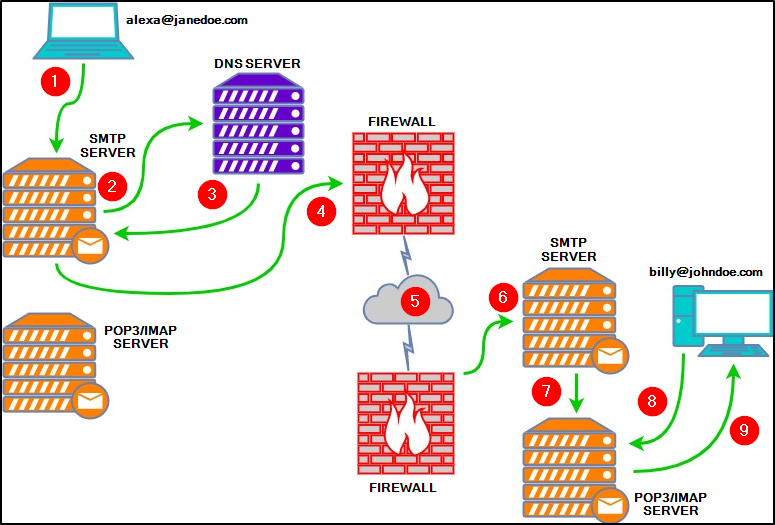
\includegraphics[width=\linewidth]{figs/email_flow.png}
    \caption{How email travels from the sender to the recipient.}
    \label{fig:c2:email_flow}
  \end{figure}

\subsection{Email structure}

Email communication is an integral component of modern digital communication, and now we know how this communication happens, understanding how an email travels from point A to point B and the protocols involved in the process. However, it is also important to understand the structure of an email and the information it contains. The standard format of email messages is known as \ac{imf}. As specified in \ac{rfc} 5322~\cite{rfc5322}, it defines the required headers and bodies for messages, as well as the content and syntax for different headers. There is also the \ac{mime} standard, which extends the capabilities of email to include multimedia content and non-ASCII text. It allows for the formatting of multipart messages and the inclusion of various types of binary files like images and documents. 
%\ac{mime} is defined in \ac{rfc} 2045~\cite{rfc2045}, \ac{rfc} 2046~\cite{rfc2046}, \ac{rfc} 2047~\cite{rfc2047}, \ac{rfc} 4288~\cite{rfc4288}, and \ac{rfc} 4289~\cite{rfc4289}.

Such protocols and formats led to the development of various email storage and exchange formats, notably \ac{eml} and \ac{mbox}. These formats utilize the foundational principles of these protocols to manage and store email data effectively.

% informação do livro https://www.dpconline.org/docs/technology-watch-reports/739-dpctw11-01-pdf/file
The \ac{eml} format typically stores each email message as an individual file, incorporating the standardized headers and body prescribed by the \ac{imf}. Attachments in \ac{eml} files are either included as \ac{mime} content within the message or referenced as separate files. \ac{mbox} combines all the emails in a folder into a single file. Although \ac{eml} and \ac{mbox} have gained widespread acceptance as standard formats because of their interoperability with current email clients, their approaches to email storage are different. Considering that \ac{mbox} is a method that keeps several emails in a file, handling each one separately may provide issues, while the individual file storage in \ac{eml} offers more granularity.
Also, it is appropriate to address the \ac{pst} format, which is primarily utilized by Microsoft Outlook. \ac{pst} files contain not just emails but also contacts, tasks, notes, and calendar events all in one file.

The selection of email format is crucial for efficient data administration and analysis when creating a system for phishing email detection. The decision to choose the \ac{eml} format over \ac{mbox} is motivated by the particular advantages it provides, especially about the granularity, providing large information about an email. The standardized nature of \ac{eml} files ensures broad compatibility with a variety of email clients beyond Microsoft Outlook, which is not the case with the \ac{pst} format. For a phishing email detection system that would need to process data from several sources, this compatibility is essential.

%estrutura de um email
\ac{eml} files include all of the raw data that makes up an email, including the message content and headers. The email headers contain details about the email servers that carried the email, thus serving as a digital trail of the email's journey from sender to recipient. This header is not just a single entity but a collection of various fields, each holding specific information.  Header fields are lines beginning with a field name, followed by a colon (":"), and followed by a field body, as specified in \ac{rfc} 5322~\cite{rfc5322}. The field name identifies the type of information, and the field body, following the colon, contains the specific details corresponding to the field name.
An example of an email headers message as an \ac{eml} file can be found in Figure \ref{fig:c2:eml}. Several fields are present in the email headers, each with its own purpose:

\begin{enumerate}[label=\Alph*]
    \item \textbf{Delivered-To}: The intended recipient's email address is contained in this email header field;
    \item \textbf{Received By}: This field contains the details of the last visited \ac{smtp} server, where the information revealed is the Server's IP address, \ac{smtp} ID of the visited server, and data and time at which the email was received by the \ac{smtp} server;
    \item \textbf{X-Received}: This field shares the IP address of the message-receiving servers, the \ac{smtp} ID of the server, and the date and time at which the email was received;
    \item \textbf{Return Path}: The return path is an email header that tells \ac{smtp} servers where they should send non-delivery notifications. According to RFC 5321,~\cite{rfc5321}, the return path consists of the sender’s mailbox;
    \item \textbf{Received From}: It has some information about the IP address of the sender along with other details like the hostname. Every server that handles this mail adds this header;
    \item \textbf{Received-SPF}: The system forwards the message only after the sender's identity is authenticated with the \ac{spf}. \ac{spf} is designed to verify that the sending server is authorized to send emails on behalf of the domain in the "From" address. It uses the domain address for authentication and adds the check status in the header field; 
    \item \textbf{Authentication Results}: \ac{mtas} apply a slew of authentication techniques to the email messages before processing them and add the results to this header field. It shares the ID of the authentication-performing server, the authentication techniques along their results;
    \item \textbf{From}: This field contains the sender's email address, indicating who sent the email;
    \item \textbf{To}: This field contains the recipient's email address;
    \item \textbf{Subject}: The subject line of the email offers a summary or a title to the email's content;
    \item \textbf{Date}: This indicates when the email was sent, providing a timestamp for the communication;
    \item \textbf{Message-ID}: It is the email's distinct ID that allows for differentiation. The same message ID cannot be shared by two emails;
    \item \textbf{MIME-Version}: This demonstrates that the message is prepared with the Multipurpose Internet Mail Extension (MIME) and supports a variety of forms, including audio, video, and plain text files.
\end{enumerate}

Depending on the email delivery service, custom headers can be included and are called X-Headers. The primary purpose of X-headers is to address the specific requirements of the sender that are not covered by the standard headers.

%eml file example

\begin{figure}[H]
  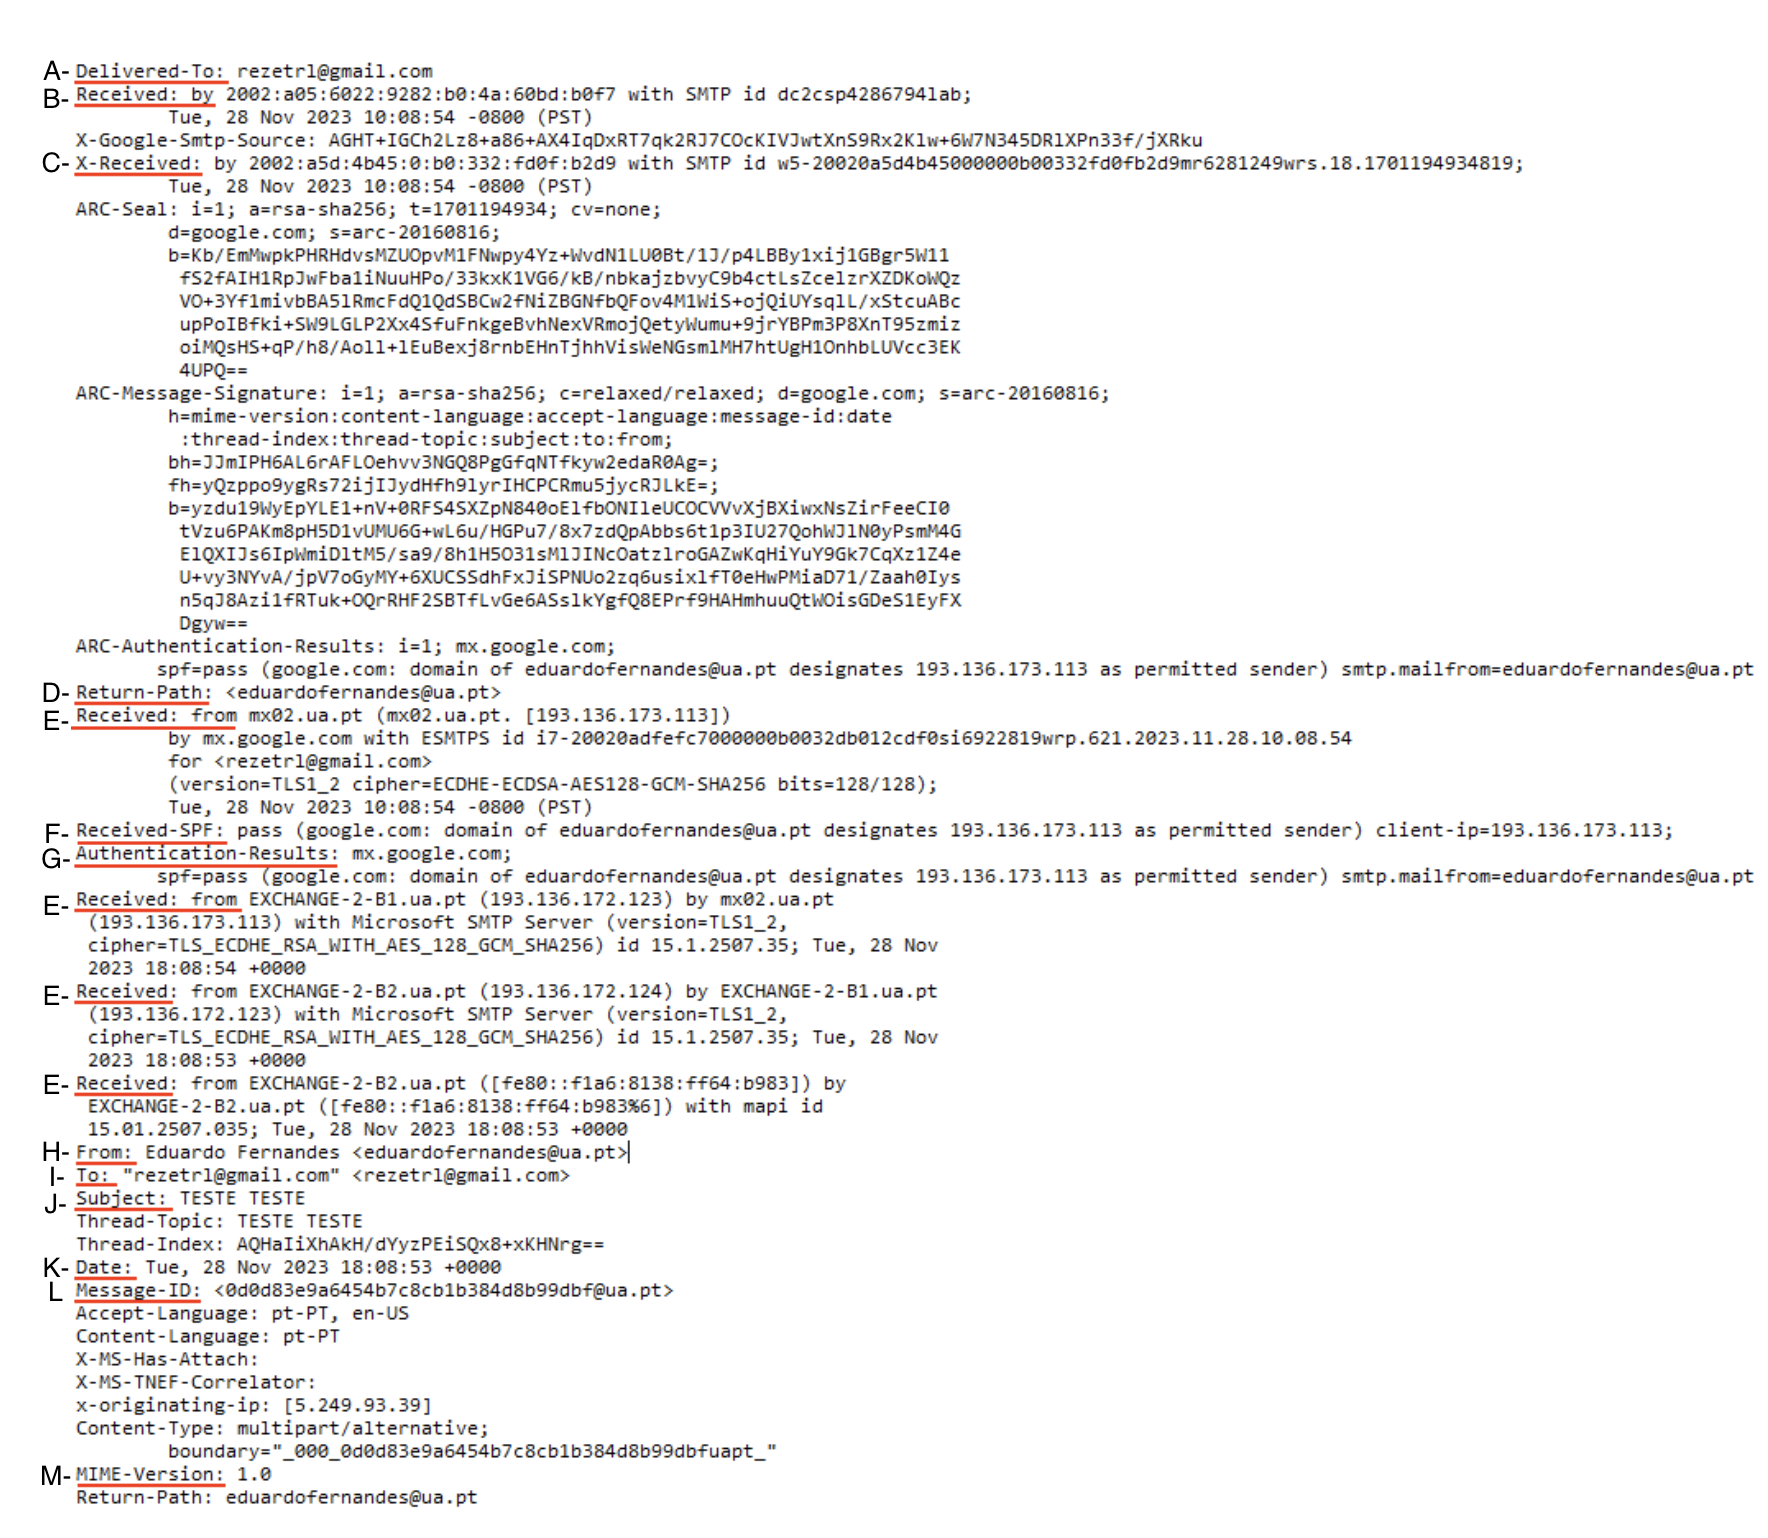
\includegraphics[width=\linewidth]{figs/eml.png}
  \caption[EML file example]{Email headers as an \ac{eml} file example.}
  \label{fig:c2:eml}
\end{figure}

As was discussed previously, the email content offers a wide range of information that can be crucial for detecting phishing emails. Besides the headers, the email body also contains equally pivotal information for detecting phishing attempts. While the email headers provide critical metadata, the body of an email often contains the substantive content that is essential for a more comprehensive analysis.

Contents of the email body are described by its \textbf{Content-Type} field, which indicates the respective formats of the information. The structure of the \textbf{Content-Type} consists of a \textbf{type} and a \textbf{subtype}, two strings, separated by a ‘/’, where no space is allowed between them. The type represents the category and can be a discrete or a multipart type, and the subtype is specific to each type. Discrete types are types that represent a single file, such as a single text or music file, or a single video. A document that is divided into several separate sections, each of which could have its own unique MIME type, is represented by a multipart type.

The list of discrete types is long but some important content-types are mentioned below:

\begin{itemize}
    \item \textbf{text}: Represents format which is human-readable. Includes subtypes such as "text/plain", "text/html", "text/css", and "text/javascript";
    \item \textbf{image}: Represents image of any type. Common subtypes examples are "image/jpeg", "image/png", and "image/svg+xml";
    \item \textbf{audio}: 	Represents any audio file format. Subtypes examples include "audio/mpeg", and "audio/wav";
    \item \textbf{application}: Represents any kind of binary data. Generic binary data is represented with the "application/octet-stream" subtype. Other common examples include "application/pdf", and "application/zip".
\end{itemize}


\begin{figure}[H]
    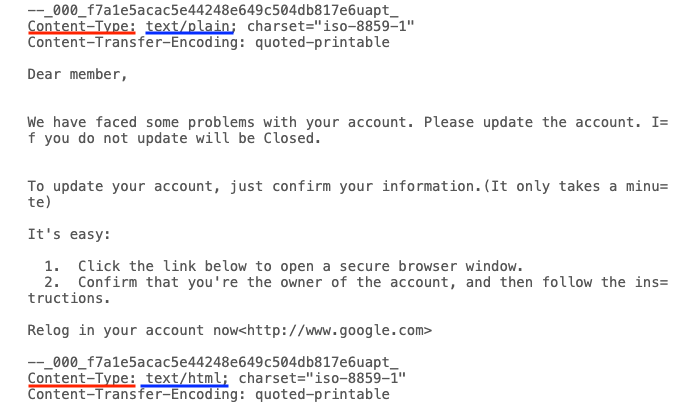
\includegraphics[width=\linewidth]{figs/eml_body.png}
    \caption{Email body in an \ac{eml} file example.}
    \label{fig:c2:eml_body}
  \end{figure}


\begin{comment}
The EML (Email) is a common format for all types of email software. We can think of the
EML file as a file generated after the email is archived, retaining the original HTML format and title, and so forth. The basis of our detection system is the EML file, which provides us with large email-related information. Fortunately, most mail systems provide a window to download EML files directly. Besides, when the user logs in to the mailbox client, the EML file is automatically downloaded to the local.
Each EML file has a standard format, which allows it to load by specified rules. In the EML file, some of the information is base64 encrypted, so it needs to be decrypted to get the rawest data. In the process of extracting, the email file that missing field values will be considered abnormal data and be discarded.
\end{comment}

\subsection{Email features for phishing detection}

% perceber o que faz com que as pessoas caiam em phishing (tecnicas de phishing e que metadados podem ajudar nestas tecnicas)

Email metadata plays a critical role in the field of email phishing detection. All the fields explained before, including headers and other structural components, can offer information to determine the authenticity of an email. This metadata, which users frequently ignore, includes details such as the sender's address, routing information, timestamps, and more, giving information to help comprehend an email's origin and path.

Email spoofing is a very common type of phishing technique. It is a threat that involves sending email messages with fake information on email headers. Because a spoofed email and regular mail are similar in many aspects, email spoofing takes advantage of these similarities. Attackers can customize the information in several fields such as "Return-Path", "Reply-To", "From", "Subject", "Date", and "To".
The "Return Path" is where bounce messages go if the email fails to deliver. In legitimate emails, the "From" and "Return-Path" are typically consistent, representing the same source. However, in the case of email spoofing, there is often a discrepancy between these two fields. Scammers frequently manipulate the "From" address to appear as a trustworthy source, although they forget to modify the "Return-Path".
One of the main warning signs is an inconsistency between the "Reply-To" and "From" addresses. This disparity suggests the sender might be attempting to hide their true identity, which is a common phishing attempt approach. Additionally, if the “From” address does not align with the entity the email claims to represent, it further raises even more questions about the email's credibility. 
Another important detail is the nature of the "Subject" line. Phishing emails frequently have subject lines that are concerning, urgent, or too appealing in an attempt to get the receiver to act immediately without closely examining the legitimacy of the email. 
The "Date" field also needs to be taken into consideration. Attackers might use might that are not logical, including dates in the future or the past. Also, if the “To” address does not specifically name you, it can be indicative of phishing. Phishing emails often lack specific identification of the recipient, suggesting a broad targeting strategy known as mass mailings.

Another technical aspect of the email's metadata that can provide important information is the \ac{spf}. A "Fail" or "SoftFail" status from the \ac{spf} check, or a lack of \ac{spf} validation, raises serious questions about the legitimacy of the email. Also, another important point is that the IP address must line up with the sender's email service. If this does not happen, it suggests that the email may have been sent from an unauthorized or suspicious server. The "Received" fields can also provide crucial information, tracing the email's path across the internet. Unknown servers along this path, especially at the beginning or end, suggest that the email routing process may be compromised, raising the possibility of a phishing attempt.\\

% falar sobre features utilizadas em outros trabalhos

\citet{8257764} categorized the spam features into three primary groups based on the examination of the features present in the relevant studies in their literature: attachment features, payload (body) features, and header features. The header features were grouped into two classes, called email metadata and subject, and are displayed in Figure \ref{fig:c2:header_features}.

\begin{figure}[H]
    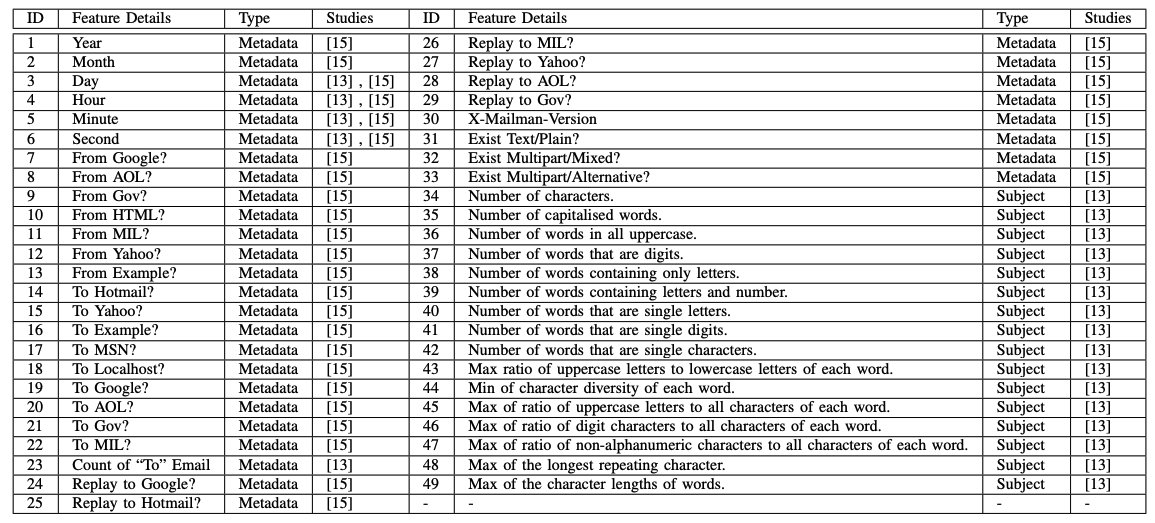
\includegraphics[width=\linewidth]{figs/headers_article.png}
    \caption{\citet{8257764} proposed header features.}
    \label{fig:c2:header_features}
  \end{figure}

\citet{Abadla202312} in their study, used a dataset that has around 3800 records and 31 features related to the body of the email message, the subject box, and the sender’s address.
The proposal highlights specific characteristics often found in phishing emails, such as the inclusion of words like "urgent" and "suspension" in the subject line. Attackers deliberately use these terms to make victims frightened and force them to act right away. In addition, they identified that phishers use header phrases like "Fwd: mail" and "Re: mail" to create the sense of a continuing conversation, which increases the possibility that the receiver may interact with the email. This analysis of header features is crucial in understanding the linguistic and psychological strategies used in phishing attacks, thereby aiding in the development of more effective detection mechanisms. They introduced also the concept of “subject richness”, which pertains to the ratio of the number of words to the number of characters in the subject line. Turns out that this feature is crucial as it influences the open rate of an email.


\begin{comment}
The first step is to understand why people fall for phishing. Something in phishing emails lures the victims into clicking on some malicious link or providing confidential information.~\citet{butavicius2022people} performed a study where the objective was to understand why that happens. For that, they conducted an online experiment, and participants underwent an email classification task designed to examine susceptibility to phishing. In the study's discussion, it was mentioned that participants phishing email detection skills were poor. They correctly identified phishing only 42\% of the time and incorrectly flagged emails that were legitimate 31\% of the time. Despite the emails having leakage cues such as poor grammar, spelling, and punctuation the majority still fell for the attack and clicked the fake malicious link provided. 
\end{comment}


% \section{Existing tools and platforms}
% ThePhish - GitHub

\section{AI for Phishing Detection}

% continual learning pode ser uma hipótese para o modelo ir aprendendo (continual learning vs reinforcement learning vs transfer learning)

As phishing techniques evolve and become increasingly sophisticated, traditional methods like rules-based filters and signature detection are no longer enough to keep us safe. This is where \ac{ml} and \ac{dl} come into play as powerful tools that can enhance our ability to detect phishing attacks. These artificial intelligence techniques enable systems to learn and adapt, allowing them to recognize subtle patterns and anomalies that may trick traditional detection approaches.
By incorporating \ac{ml} and \ac{dl} into phishing detection, we not only aim to address the difficulties of identifying these deceitful communications but also play a crucial role in strengthening cybersecurity measures.

\subsection{Natural Language Processing}

% falar de coisas gerais sem entrar muito em detalhe

% descrição do que é nlp
As a branch of artificial intelligence, \ac{nlp} focuses on the interaction between computers and human language. \ac{nlp} combines the power of linguistics and computer science to study the rules and structure of language and create intelligent systems capable of understanding, analyzing, and extracting meaning from various human inputs, such as voice, and text.

It covers a range of techniques and methodologies designed to enable machines to understand, interpret, and respond to human language in a valuable and meaningful way. Human signs and languages, such as voice, writing, and text, can be automated with a certain level of accuracy using \ac{nlp} techniques~\cite{Sathish20231612}.

% o que é que o nlp pode fazer para detetar phishing
The relevance of NLP in detecting phishing emails is based on its ability to analyze and understand the textual content of emails. Phishing emails frequently include linguistic clues different from those in normal correspondence, and trick recipients into revealing sensitive information. These cues can be subtle, such as the use of specific words or phrases, or more obvious, such as poor grammar and spelling. In either case, these linguistic features can be used to identify phishing emails and \ac{nlp} techniques can be used to extract and analyze them.

% falar do processo de nlp e de algumas técnicas utilizadas
The \ac{nlp} field is vast and has a wide array of techniques, each contributing uniquely to the understanding and processing of language in the \ac{nlp} process. Data preprocessing is one step in \ac{nlp} that involves cleaning and transforming raw data into a format that can be understood and used by models. Some of the techniques used in this step include tokenization, normalization, stemming, the use of stop words, the application of regular expressions and both syntactic and semantic analysis.
Feature extraction is another important step in \ac{nlp} that involves the extraction of features from the text. These features can be used to train \ac{ml} models to perform various tasks in this field. Techniques such as bag-of-words, word embeddings, and TF-IDF are used to extract features from text.
After this, numerical features extracted by the previous techniques can be fed into \ac{ml} models. Depending on the task, different models can be used, such as classification, clustering, and regression models.

% mostrar aplicações de nlp com machine learning
\citet{Vazhayil201869} presents an insightful application of \ac{nlp} methods in conjunction with \ac{ml} models for phishing email detection. This study uses Term Document Matrix (TDM) for the non-sequential representation of the corpus, followed by Singular Value Decomposition (SVD) and Nonnegative Matrix Factorization (NMF) to extract important features. These extracted features were then used to train various \ac{ml} algorithms, including \ac{dt}, \ac{knn}, \ac{nb}, \ac{rf}, \ac{svm}, and \ac{lr}. In the conclusion, they highlighted the effectiveness of this approach in distinguishing phishing emails from legitimate ones. However, the paper also acknowledges a limitation: the reliance on feature selection, which requires domain knowledge. To address this, future work could incorporate \ac{dl} models that can learn more complex patterns directly from the raw data, potentially improving efficacy. \citet{Gutierrez2018988} mentioned that the most common defensive approaches frequently display a lack of adaptability. This is primarily because of its basis in rigid frameworks like regular expressions that recognize specific text patterns. A major flaw with \ac{nlp} developed on \ac{ml} is their reliance on surface-level text analysis rather than exploring deeper semantics. This means that if different synonyms of words are chosen or the sentence construction is changed, it is difficult for \ac{nlp} built on \ac{ml} to analyze these changes.

% mostrar aplicações de nlp com deep learning
Advancements in this area have led to the development of more sophisticated techniques. Unlike traditional \ac{ml} models, \ac{dl} models can automatically detect and learn features from raw text, allowing them to capture complex relationships between words and phrases in a language and to generalize to new and unseen examples. Some examples of \ac{dl} models that can be used in \ac{nlp} are \ac{rnn}, \ac{cnn} and transformer models. \ac{rnn} is a type of neural network that can process sequential data, such as text, by using a hidden state to store information about previous inputs. \ac{cnn}, typically known for image processing, have also been effectively repurposed for \ac{nlp} tasks. Moreover, the emergence of Transformer models marks a significant leap. These models excel in understanding the context of language, processing each word concerning all other words in a sentence, and using self-attention mechanisms to capture the global relationships in a sentence.

% ver melhor este texto
\begin{comment}
    \citet{Gutierrez2018988} mentioned that the most common defensive approaches frequently display a lack of adaptability. This is primarily because of its basis in rigid frameworks like regular expressions that recognize specific text patterns. This limitation highlights how important it is to find different methods to improve phishing detection. The problem with already existing automated solutions, built to manage the flood of phishing emails, is to quickly detect unseen phishing attempts. A major flaw in these solutions is their reliance on surface-level text analysis rather than exploring deeper linguistic patterns and deceitful strategies, such as the use of synonyms and varied sentence structures.
    In the proposed solution they used advanced \ac{nlp} techniques like Named Entity Recognition that its used to recognize different entity types, such as persons, locations, organizations, within the text, and Freebase that essentialy returns potential categories the entity belongs to and provides a score of how relevant each category is. These two techniques form a set of higher-level features, that also includes synonym substitution, to better understand the semantics of phishing emails.
\end{comment}


\subsection{Machine Learning approaches}


The work proposed by~\citet{rabbi2023phishy} aims to find the most efficient techniques for preventing phishing attacks. For that, six ML algorithms were separated including Logistic Regression (LR), K-Nearest Neighbors (KNN), AdaBoost (AB), Multinomial Naive Bayes (MNB), Gradient Boosting (GB), and Random Forest (RF). One of the goals was to answer what is the most powerful machine learning algorithm for detecting phishing emails and the results showed that the Random Forest performed better than other ML algorithms having 98.38\% of accuracy and a low rate of false negatives. Although RF obtained better results, its training time is relatively long when compared to others. However, the approach solely focuses on the email body features. There is more information such as the sender details, header information, and URLs in the email that can provide useful information for the model and increase performance.

In their study, the authors of~\cite{Kumar2023222} introduced a phishing URL detection method that integrates multiple machine learning (ML) algorithms with unique hybrid features. These hybrid features are generated by first applying Principal Component Analysis (PCA) to word vector features, and then merging them with natural language processing (NLP) features. The dataset used in this study comprises approximately 37,000 URLs, evenly split between phishing and legitimate sites. Word vectors, also known as word embeddings, numerically represent words in a high-dimensional space. PCA is employed to reduce the dimensionality of these vectors. The resultant hybrid feature set, post-merging with NLP features, encompasses 142 distinct features. Among the various ML algorithms evaluated, the Random Forest algorithm exhibited the highest accuracy, achieving a remarkable 99.75\%.

Muhammad Shaukat et al.~\cite{Shaukat2023} proposed a solution that uses a three-layered approach to detect phishing websites. This multi-perspective layered evaluation has three layers: URL layer, text layer, and image layer. The first one analyzes URL features to detect phishing URLs, the second layer looks for spam content in website text by using natural language processing and the last one categorizes the content of websites by processing text and graphics from advertising. The PhishTank dataset containing 20,000 phishing URLs and the SMS spam and ham dataset from Kaggle were used to train the machine learning models for the first two layers. The third layer takes the images from the websites as input to convert them into text so that they can be readable and given as input to the second layer model. For the URL classification the Decision Tree, Random Forest, Multilayer Perceptron, Support Vector Machine, Logistic Regression and XG Boost models were tested. Naïve Bayes and Linear SVC models were used in the second layer to perform phishing text classification. The results showed up to 91.2\% accuracy in the detection of legitimate or phishing URLs with XGBoost, and 98.9\% accuracy with the Linear SVC model in the text analysis step.

Hadi El Karhani et al.~\cite{Karhani2023206} present a novel approach to detecting phishing URLs and SMS-based phishing (smishing) attacks. This approach combines domain-related features with natural language processing (NLP) techniques. The features related to domains are extracted and used alongside NLP, which is trained on actual smishing messages, to detect attacks accurately. The study proposes integrating this detection system with the open-source threat intelligence platform MISP (Malware Information Sharing Platform). This integration enhances the storage and utilization of flagged phishing domains.
The dataset for this study includes data from TELUS Corporation and publicly available sources, featuring a mix of phishing and legitimate domains and SMS messages. The methodology involves a hybrid model that combines a Decision Tree model and an NLP model using Support Vector Classification (SVC).
The model demonstrates an impressive accuracy of 99.40\% and an F1 score exceeding 99\%. The domain checker, part of the hybrid model, showed notable generalization capabilities with an F1 score of 99.01\% and an accuracy of 98.04\%.
The NLP checker, while effective, did not generalize as well to the confirmed phishing dataset provided by TELUS, with an F1 score and accuracy of 92.98\% and 86.88\% respectively.
When both models were combined, the NLP checker effectively corrected 69.35\% of the domain checker's false negatives, improving the final accuracy to 99.40\%.

The importance of this work lies in its high accuracy and practical application in real-time phishing detection. The integration with MISP and the combination of domain and NLP features represent an effective approach to tackling phishing threats.

\subsection{Deep Learning approaches}

The authors of~\cite{Benavides-Astudillo2023} developed a phishing detection model focusing on the text of web pages rather than URL addresses. This model uses Natural Language Processing (NLP) and Deep Learning (DL) algorithms, specifically using the Keras Embedding Layer with Global Vectors for Word Representation (GloVe) to exploit semantic and syntactic features of webpage content. The method involves four phases: word parsing, data pre-processing, feature representation, and feature extraction. This approach ensures that important words and the order in which they appear are both considered for analysis.
The model's performance was evaluated using four DL algorithms: Long Short-Term Memory (LSTM), Bidirectional LSTM (BiLSTM), Gated Recurrent Unit (GRU), and Bidirectional GRU (BiGRU). Notably, all four algorithms achieved a mean accuracy of at least 96.7\%, with BiGRU emerging as the top performer, achieving an accuracy of 97.39\%.
Further analysis revealed that both GRU and BiGRU consistently outperformed LSTM and BiLSTM in terms of test accuracy. Notably, GRU demonstrated the fastest training time, completing its training in just 240 seconds, which could be beneficial if rapid processing is required.

\section{Sentiment analysis}

% o que é sentiment analysis
Sentiment analysis is a \ac{nlp} technique that refers to the process of evaluating and determining the sentiment, which is characterized as feeling or emotion, contained in a certain text.
The core of sentiment analysis lies in polarity detection, which classifies text into basic categories like positive, negative, or neutral. However, sentiment analysis goes beyond polarity to identify particular emotions like happiness, frustration, anger, and sadness. This technique can be applied to a wide range of domains, including social media, customer reviews, and emails.

% como funciona sentiment analysis (ver aqui https://monkeylearn.com/sentiment-analysis/)
Generally, the input to a sentiment classification model is a piece of text, and the output is the probability of a certain sentiment or emotion. Typically, this probability is based on either hand-generated features, word n-grams, TF-IDF features, or using deep learning models to capture sequential long- and short-term dependencies. Many emotion systems use lexicons, which are lists of words and their corresponding emotions. These lexicons can be used to determine the sentiment of a text by counting the number of words that match the words in the lexicon. However, this approach is limited by the fact that it does not consider the context of the words, which can lead to inaccurate results.

% desafios de sentiment analysis
Despite its wide applications, sentiment analysis faces several challenges. One of the most significant is detecting sarcasm and irony, as these often convey the opposite meaning of the literal words used, leading to potential misinterpretation. Additionally, sentiment analysis must contend with contextual and cultural variations. The same phrase may carry different meanings in different cultures or situations, complicating universal model applicability. Moreover, because human language can be unclear and different people might see it differently, sentiment analysis becomes more complicated. What is considered a positive sentiment in one context may be neutral or even negative in another, which is why we need advanced models that understand the context.

% téncicas de sentiment analysis


% exemplos de artigos que fazem sentiment analysis
% ver melhor esta parte
The~\citet{SAILUNAZ2019101003} study provides a robust example of an integrated approach. The researchers focused on extracting sentiment and emotion from tweets and replies on specific topics. This involved creating a dataset encompassing text, user emotion, sentiment information, and various other parameters.

A specific example is the Sentiment Analysis Module detailed in the~\citet{10085351} study, where this module captures the emotions or sentiments expressed in emails. It employs the \ac{nltk}, an open-source Python library, to analyze the text based on common and repetitive sentiment words included in the training set. Determining sentence polarity is an important part of this module since it helps to comprehend the emotional tone that an email provides. The system pre-determines the polarity of specific polar words to interpret the sentiment accurately. 



\section{Insights}

No tool detects phishing emails and also the sentimental analysis of the email.

A model that continually adapts to new sophisticated phishing strategies is important to deceive this type of attack. Transformers are a type of deep learning model that can automatically learn, adapt, and identify phishing emails based on their behaviors.
\chapter{Methodology}
\label{chapter:methodology}


to do...
%\chapter{Methodology}
\label{chapter:methodology}


to do...
%\chapter{Work done}
\label{chapter:work_done}

\section{Metadata Analysis}

Um dos desafios enfrentados na luta contra ataques de phishing é a obsolescência dos datasets atualmente disponíveis. Muitos desses conjuntos de dados não refletem as técnicas e estratégias mais recentes utilizadas, tornando as ferramentas de detecção menos eficazes contra novos ataques. Para superar este problema, propôs-se a criação de um dataset sintético que incorpore as características dos ataques de phishing mais recentes.

Inicialmente, foi necessário recolher uma coleção de e-mails de phishing reais e recentes. Esses e-mails servem como base para entender as tendências atuais e as técnicas utilizadas pelos phishers. A análise dos metadados desses e-mails é crucial, pois oferece insights sobre padrões comuns que podem ser replicados de forma sintética para enriquecer o dataset. Os metadados recolhidos incluem, mas não se limitam a, o endereço de e-mail do remetente, o destinatário, o assunto do e-mail, a data de envio, além de outros campos que podem revelar padrões de comportamento dos atacantes. Essas informações são essenciais para criar um modelo realista de headers de e-mail.

Com o auxilio de bibliotecas de python, desenvolveu-se um script capaz de gerar headers de e-mail fictícios. Este script utiliza os metadados extraídos dos e-mails reais como referência para criar headers convincentes que imitam autenticamente os utilizados em campanhas de phishing. A geração de headers fictícios inclui a manipulação cuidadosa de campos como o remetente, o destinatário e a data, de modo que os e-mails sintéticos pareçam plausíveis aos sistemas de detecção baseados em análise de metadados.

No final o objetivo é possuir um dataset de e-mails de phishing sintéticos que possam ser utilizados neste contexto de análise de phishing.
Este conjunto de dados será utilizado em dois principais modelos analíticos:
\begin{itemize}
    \item \textbf{Modelo de análise de headers:} Este modelo visa analisar os metadados dos e-mails para identificar padrões comuns e características distintivas dos e-mails de phishing. A análise dos headers é fundamental para a detecção de e-mails maliciosos, uma vez que muitas vezes os atacantes utilizam técnicas de spoofing para enganar os destinatários.
    \item \textbf{Modelo de análise de texto:} Este modelo visa analisar o conteúdo dos e-mails para identificar padrões de linguagem, estilo e conteúdo associados a e-mails de phishing. A análise do texto é crucial para a detecção de e-mails maliciosos, uma vez que os atacantes muitas vezes utilizam técnicas de engenharia social e manipulação psicológica para enganar os destinatários.
\end{itemize}

\section{Text Analysis}
TDB

\section{Emotion Analysis}

Após a análise da literatura cheguei a conclusão que modelos pré treinados apresentavam boas métricas e que poderiam ser utilizados na análise de emoções de um e-mail. 
Inicialmente, tive como primeira opção um modelo pré treinado chamado de XLMRoBERTa, que é um modelo de linguagem que foi treinado em 2.5TB de dados de texto de diferentes línguas, o que parecia ser uma vantagem no inicio para a análise de emoção em e-mails de lingua portuguesa.
No entanto, após a análise de mais alguns modelos pré treinados, descobri um modelo baseado no RoBERTa, que foi fine-tuned com textos de Reddit anotados com emoções para a tarefa de classificação de emoções.
Apesar deste modelo apresentar a vantagem de ter sido treinado especificamente para a tarefa de classificação de emoções, o modelo foi treinado em textos em inglês, o que poderia ser um problema para a análise de e-mails em português. Chegou-se á conclusão que no caso de e-mails portugueses poderia-se utilizar uma ferramenta de tradução para inglês e posteriormente analisar a emoção do e-mail.

Devido a falta de um dataset de e-mails anotados com emoções, foi necessário criar um para o desenvolvimento deste modelo. 
Primeiramente, foram reunidos 100 emails e os mesmos foram anotados com emoções para testar a performance do modelo quando aplicado a e-mails. Foram obtidas algumas métricas como \textit{accuracy}, \textit{precision}, \textit{recall} e \textit{f1-score}. Abaixo encontra-se uma tabela com os resultados obtidos juntamente com a performance do modelo quando aplicado a textos de Reddit.

\begin{table}[ht]
    \centering
    \begin{tabular}{p{7cm}p{1.5cm}p{1.5cm}p{1.5cm}p{1cm}}
    \hline
    \textbf{Overall Metrics} & \textbf{Accuracy} & \textbf{Precision} & \textbf{Recall} & \textbf{F1-Score} \\
    \hline
    \textit{Reddit text performance results (multilabel prediction with threshold of 0.5)} & 0.474 & 0.575 & 0.396 & 0.450 \\
    \hline
    \textit{E-mail text performance results (using top1 classification)} & 0.371 & 0.470 & 0.372 & 0.385 \\
    \hline
    \hline
    \textit{E-mail text performance results (using multilabel prediction with threshold of 0.5)} & 0.324 & 0.404 & 0.338 & 0.349 \\
    \hline
    \end{tabular}
    \label{tbl:c4:results_table}
    \end{table}

O modelo, treinado nas emoções do Reddit, não tem um desempenho tão bom em textos de e-mail, indicando um problema de generalização. Os estilos linguísticos e as expressões emocionais nos e-mails provavelmente diferem significativamente daqueles encontrados nos comentários do Reddit.

Para melhorar estes resultados seria necessário treinar o modelo com um dataset de e-mails anotados com emoções. Um dataset com as caracteristicas pretendidas para este trabalho não existe (um dataset com e-mails anotados com emoções como medo, surpresa, curiosidade,...), o que torna a tarefa de treinar um modelo para a análise de emoções em e-mails mais complexa. De modo a progredir com o desenvolvimento do modelo, foram tomadas duas medidas para resolver este problema:
\begin{itemize}
    \item Anotar e-mails manualmente com a ajuda de colegas e com o auxilio de uma LLM (Large Language Model) para a tarefa de geração de e-mails;
    \item Utilizar um ciclo de active learning para treinar o modelo.
\end{itemize}

A primeira medida envolveu a anotação manual de e-mails. Dada a escassez de datasets disponíveis com e-mails categorizados por emoções específicas, como medo, surpresa e curiosidade, tornou-se essencial criar um conjunto de dados inicial próprio. Para isso, contamos com a colaboração de colegas e o auxílio de um Modelo de Linguagem de Grande Escala (LLM) denominado Mixtral, para gerar textos de e-mails realísticos com base nos 100 e-mails previamente anotados. Com isto, foram gerados cerca de 400 e-mails anotados com emoções, que posteriormente foram retificados por mim, formando assim um dataset de 500 e-mails anotados. Esta etapa é fundamental para estabelecer uma base sólida de dados anotados que refletisse as nuances e a diversidade das expressões emocionais em e-mails. A próxima fase seria dividir estes e-mails e pedir a colegas para anotar manualmente os mesmos com emoções, garantindo assim que o modelo tivesse exemplos precisos e relevantes para iniciar o treinamento.

A utilização de um ciclo active learning é essencial devido à escassez de e-mails anotados com emoções disponíveis para treinamento. Este método é particularmente útil em cenários onde os dados anotados são limitados ou caros de obter, como é o caso dos e-mails categorizados por emoções.
Este ciclo permite que o modelo seja treinado de maneira mais eficiente, maximizando o impacto de cada exemplo anotado. Inicialmente, o modelo é treinado com um conjunto pequeno de dados anotados. Após essa fase inicial, o modelo é usado para fazer previsões em um conjunto de dados não anotados. Em seguida, apenas as instâncias sobre as quais o modelo tem menos certeza — ou seja, aquelas que ele considera mais complicadas de classificar — são selecionadas para anotação manual.
Este processo não só ajuda a melhorar a precisão do modelo com um menor volume de dados, como também direciona o esforço de anotação para os exemplos que mais contribuirão para o aprendizado do modelo. Assim, cada ciclo de anotações e treinamentos subsequentes torna o modelo progressivamente melhor em identificar e classificar emoções em e-mails, otimizando tanto os recursos como o tempo de desenvolvimento.

Ambas as medidas são complementares e essenciais para o desenvolvimento de um modelo robusto e eficaz para a análise de emoções em e-mails. A anotação manual cria um ponto de partida confiável, enquanto o ciclo de active learning assegura que o modelo evolua e se adapte com o máximo de eficiência. Juntas, estas estratégias ajudam a superar as limitações impostas pela falta de dados pré-existentes e são fundamentais para a construção desta ferramenta de análise de emoções.


Abaixo encontra-se umas imagens que traduzem um exemplo do processo de active learning, onde é possível ver a evolução do modelo ao longo de 2 iterações. 

\begin{figure}[H]
    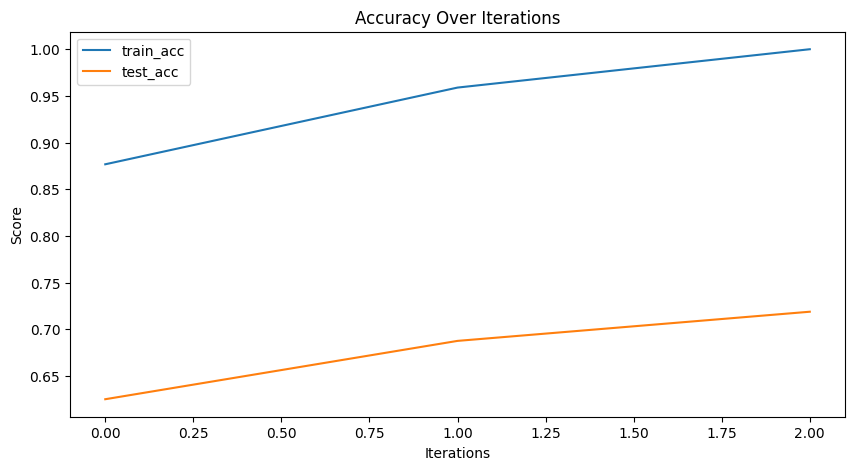
\includegraphics[width=\linewidth]{figs/active_learning.png}
    \caption{Active learning cycle through two iterations.}
    \label{fig:c4:active_learning}
  \end{figure}

A abordagem de active learning é aplicada para melhorar iterativamente o modelo, adicionando exemplos novos e informativos ao conjunto de treinamento. A modesta melhoria na precisão dos testes mostra que a aprendizagem activa está a contribuir para um melhor desempenho do modelo. No entanto, a diferença entre a precisão do treino e do teste ainda é significativa, o que sugere que o modelo pode estar a sofrer de sobreajuste. Esta disparidade geralmente indica que o modelo está a aprender a memorizar os dados de treino, incluindo ruídos e detalhes não aplicáveis ​​a casos gerais. Para mitigar este problema, é necessário analisar o erro do modelo e identificar quais emoções não estão a ser corretamente identificadas e porquê. Além disso, é importante incluir mais exemplos que desafiem o modelo e o forcem a generalizar melhor. A implementação de técnicas como data augmentation, dropout e regularização também pode ajudar a evitar o sobreajuste e melhorar a generalização do modelo.


NEXT STEPS:
\begin{itemize}
    \item Analise de erro do modelo para identificar quais sao as emoções e o porque de não serem corretamente identificadas;
    \item Incluir mais exemplos que desafiem o modelo e o forcem a generalizar melhor;
    \item Implementar data augmentation para aumentar a diversidade dos dados de treino para evitar overfitting;
    \item Implementar métodos como dropout e regularização para evitar overfitting;
\end{itemize}

%%%%%%%%%%%%%%%%%%%%%%%%%%%%%%%%%%%%%%%%%%%%%%%%%%%%%%%
% End of Thesis text 
%%%%%%%%%%%%%%%%%%%%%%%%%%%%%%%%%%%%%%%%%%%%%%%%%%%%%%%

\backmatter

%%%%%%%%%%%%%%%%%%%%%%%%%%%%%%%%%%%%%%%%%%%%%%%%%%%%%%%
% Print all used references
%%%%%%%%%%%%%%%%%%%%%%%%%%%%%%%%%%%%%%%%%%%%%%%%%%%%%%%

\begingroup
\renewcommand{\bibfont}{\footnotesize}
% Redefine References name to Portuguese
% Change if you are using english
\defbibheading{bibliography}[Referências]{
	\chapter{#1}
}
\SingleSpacing
\setlength\bibitemsep{8pt}
\printbibliography[heading=bibliography]
\endgroup


%%%%%%%%%%%%%%%%%%%%%%%%%%%%%%%%%%%%%%%%%%%%%%%%%%%%%%%
% Load appendix
%%%%%%%%%%%%%%%%%%%%%%%%%%%%%%%%%%%%%%%%%%%%%%%%%%%%%%%

\mainmatterWithoutReset
\appendix

% \include{appendix-a}
% \include{appendix-b}
% \include{appendix-c}

\end{document}
